\documentclass[conference]{IEEEtran}
\IEEEoverridecommandlockouts
% The preceding line is only needed to identify funding in the first footnote. If that is unneeded, please comment it out.
\usepackage{cite}
\usepackage{amsmath,amssymb,amsfonts}
\usepackage{algorithmic}
\usepackage{graphicx}
\usepackage{textcomp}
\usepackage{xcolor}
\usepackage{listings}
\usepackage{siunitx}
\def\BibTeX{{\rm B\kern-.05em{\sc i\kern-.025em b}\kern-.08em
    T\kern-.1667em\lower.7ex\hbox{E}\kern-.125emX}}
\begin{document}

\title{Radio Society Defense Network Preliminary Report}

\author{\IEEEauthorblockN{Oliver Trevor}
\IEEEauthorblockA{\textit{Department of Electrical Engineering and Computer Science} \\
\textit{Massachusetts Institute of Technology}\\
Cambridge, USA \\
olt@mit.edu}}

\maketitle

\begin{abstract}
We present a design for a real-time radio transceiver fingerprinting system for preventing undesirable users from being able to retransmit their signal on amateur radio repeaters. The system, which is implemented on an FPGA fabric using minimal external signal processing, digitizes the raw demodulated FM signal from a repeater's input frequency and recognizes the characteristic frequency deviations caused by the initial instability in most FM transceiver's PLLs. We will evaluate system performance using radios of known identity to track how often the system can correctly identify a transceiver.
\end{abstract}

\begin{IEEEkeywords}
Field programmable gate arrays, Radio, Transceiver identification, Matched filtering, Digital signal processing
\end{IEEEkeywords}

\section{Analog Design}

\begin{figure}
    \centerline{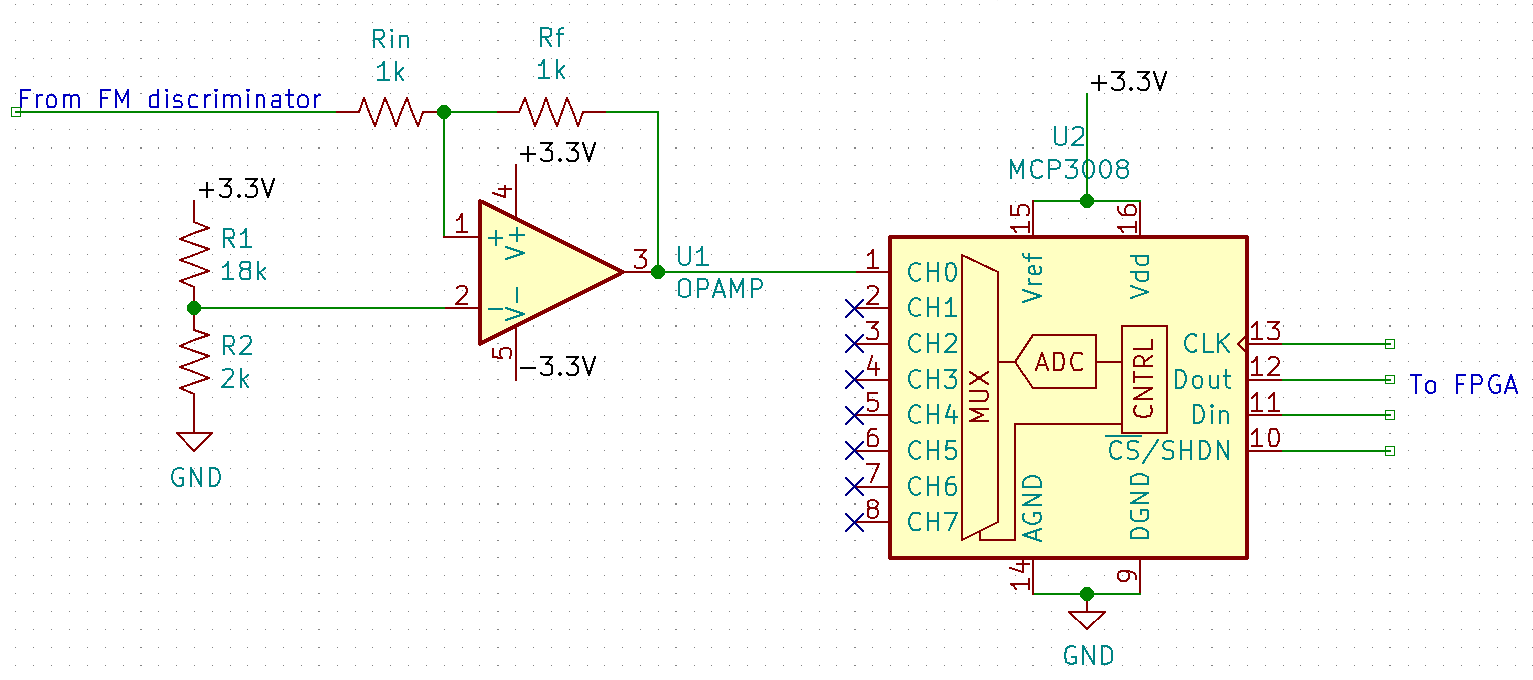
\includegraphics[width=0.5\textwidth]{Analog_Design.png}}
    \caption{Analog frontend design}
    \label{analog_frontend_design}
\end{figure}

The analog frontend uses a single MCP6002 op-amp to add a DC offset and scale factor to the incoming signal (which has no DC offset). This allows the MCP3008 SPI ADC to digitize the waveform, as it is not capable of reading voltages significantly below its ground. The op-amp also gives us the option of adding analog gain to better utilize all the bits of the ADC. As a side effect of this topology, the incoming signal is inverted, but that does not affect fingerprinting. The transfer function of the circuit (shown in Fig.~\ref{analog_frontend_design}) is:

\begin{equation*}
    v_o = (\SI{3.3}{V}) \left( \frac{R_2}{R_1 + R_2} \right) \left( \frac{R_f + R_{in}}{R_{in}} \right) - \frac{R_f}{R_{in}} v_{in}
\end{equation*}

Note that, since we currently sample the ADC at 52.6312 kSps, no analog anti-aliasing signal is required, as there are not any significant spectral components past the Nyquist frequency.

\section{Digital Architecture}

\subsection{Input and Output}

The \lstinline{spi_controller} submodule of the \lstinline{mcp3008_adc} module implements a simple FSM that shifts data from the AXI bus out over SPI while shifting data in and sending it out over the AXI bus. Data is latched on the falling edge of the SPI clock to maximize the time the line has to ``settle" before the MCP3008 samples it on the rising edge of the SPI clock. Currently, the SPI clock is 10 MHz, and each SPI transaction lasts 17 bits. This ends up resulting in a 52.6312 kSps sampling rate.

Another simple FSM implements a UART output at 115200 baud on the PMOD connectors with 8 data bits per transaction, 1 start bit, 1 stop bit, and 1 odd parity bit. This allows quickly exporting recorded waveforms to a Python program on a computer over an FTDI cable for debugging and analysis.

The UART will also output classification results from the matched filters. There will also be a binary ``transmit enable" signal for a repeater controller to enable banning specific users by their fingerprints.

The \lstinline{spi_controller} module for the ADC will also be re-used for a module that communicates with a microSD card in SPI mode. A fixed number of fingerprints of fixed length will be stored directly on the microSD card starting at address zero to obviate the need for a filesystem. A large FSM will implement the initialization and block read commands from the SD card specification, then send the stored data out over the AXI bus to the filter manager FSM when the FPGA is reset.

\subsection{Transmission Detection}

Since it is not possible to run a large number of matched filters fast enough to run them continuously (i. e. running the entire matched filter set on the last $ N $ samples in the time between incoming ADC samples), the system instead has to \emph{trigger} on a detected incoming transmission, record it, then process and classify it before the repeater user starts speaking. The triggering algorithm maintains a ring buffer in a BRAM of the last 50 samples. After each sample, the algorithm finds the minimum and maximum of the ring buffer. Due to the effect known as \emph{FM quieting}, the difference between the maximum and minimum (essentially a crude approximation of the envelope of the demodulated signal) will drop sharply when a transmission begins and the incoming signal ``captures" the receiver. A Schmitt trigger detects this sharp drop and outputs a trigger signal to tell another module to start storing the incoming samples into a longer buffer.

For testing purposes, the trigger signal is also routed out to a digital pin so that an external oscilloscope can trigger off of it. A successful capture is shown in Fig.~\ref{keyup_oscilloscope}. The same signal exported from the FPGA's BRAMs via the UART and graphed on a computer is shown in Fig.~\ref{keyup_fpga}.

\begin{figure}
    \centerline{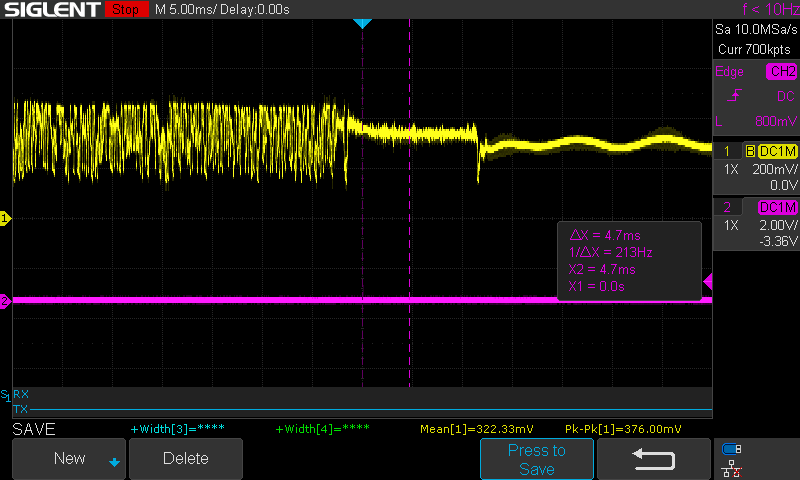
\includegraphics[width=0.5\textwidth]{First_Working_Capture_Oscilloscope.png}}
    \caption{FT-3D keyup recorded on Siglent SDS1204X-E oscilloscope, triggered using FPGA. The trigger signal on channel 2 (the purple signal) is barely visible as an impulse in the middle of the display.}
    \label{keyup_oscilloscope}
\end{figure}

\begin{figure}
    \centerline{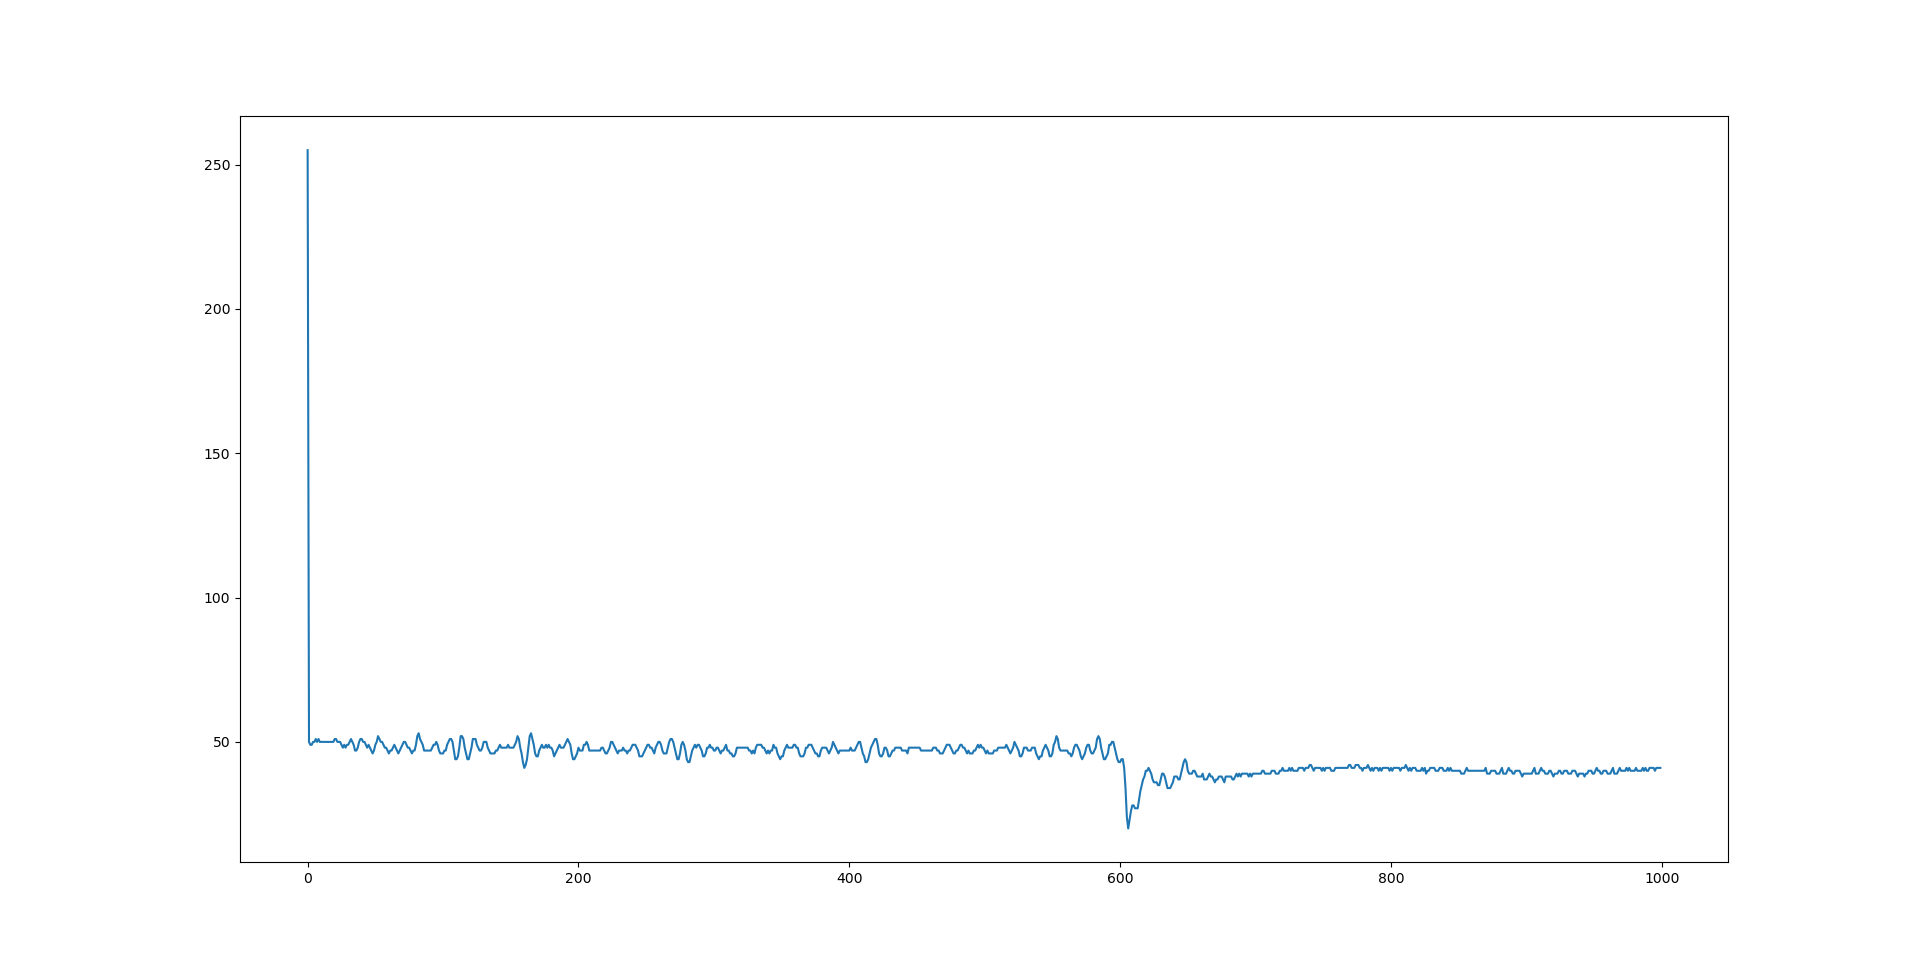
\includegraphics[width=0.5\textwidth]{First_Working_Capture_FPGA.png}}
    \caption{FT-3D keyup recorded on FPGA and exported over UART to computer. Note the similar characteristic ``triple decaying peaks" feature of this radio visible in both the oscilloscope and FPGA captures.}
    \label{keyup_fpga}
\end{figure}

\subsection{Matched Filtering}

The matched filter modules perform a simple correlation between the incoming signal and a stored fingerprint signal by sliding one across the other and computing their dot products at each point. The correlation score is the maximum dot product. Since correlations require a zero-mean signal, the stored fingerprint is preprocessed by a Python script to subtract out an DC bias. The incoming waveform must be averaged (and that average subtracted from the sample values to produce signed values from unsigned ones) by the matched filter module.

\section{Evaluation Results}

Capturing signals works and produces signals that are visually similar to those captured by an actual oscilloscope. Although the matched filtering module is mostly done and appears to work, the matched filter management module that feeds the captured signals to the filters is not, so it was not yet possible to test the matched filters in hardware.

However, feeding actual recorded signals from the UART into the matched filter testbench shows that it can differentiate between radios effectively. Two recordings of an FT-70D radio have a maximum correlation score of 2 million, whereas a recording of an FT-70D radio against an FT-3DR had a maximum correlation score of 250,000. The latter is shown in Fig.~\ref{correlation}.

\begin{figure}
    \centerline{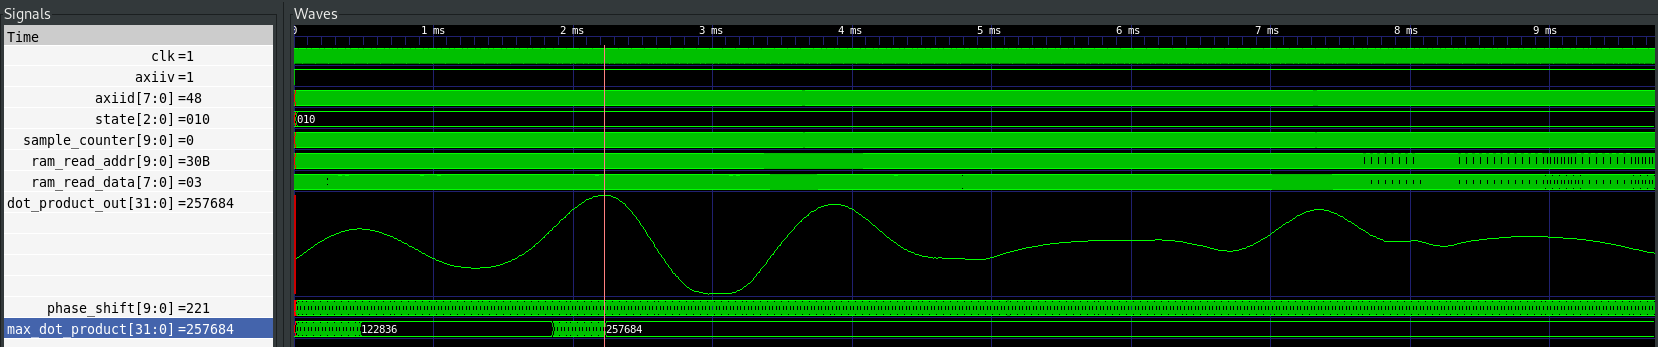
\includegraphics[width=0.5\textwidth]{FT70D_vs_FT3DR.png}}
    \caption{GTKWave visualization of output of matched filter correlating a reference fingerprint of an FT-70D radio against an FT-3DR. The \lstinline{dot_product_out} signal shows the correlation waveform.}
    \label{correlation}
\end{figure}

\section{Instrumentation and Testing}

We used a Siglent SDS1204X-E digital storage oscilloscope to obtain initial recordings of various radios' keyup characteristics to develop the matched filtering in Python and determine what sampling rate/bit depth would be required to accurately reproduce the signals. A custom C program from a previous project for converting oscilloscope binary dump files into CSV files was extremely useful.

We also used a Siglent SDG2042X arbitrary waveform generator to generate repeatable test waveforms to ensure that the ADC was digitizing incoming signals correctly.

A Python script that recorded and stored exported signals from the FPGA's UART over an FTDI cable allowed us to easily run testbenches in Icarus Verilog against the exact signals as the FPGA would see them. This was extremely useful for verifying and debugging DSP algorithms. Additionally, it allowed us to generate ROMs of actual fingerprint signals and synthesize them into the design's matched filtering stage for testing the filters without having to load the data from the microSD card.

Most of the DSP algorithms were prototyped in Python and C both to develop them more easily and to provide a reference implementation to compare the output of Verilog testbenches to.

Each module in the design had its own testbench (some which used \lstinline{$readmemh()} to load memory files generated from actual recorded signals from the UART), as well as small Bash scripts to run the testbenches and open GTKWave with the appropriate display configuration. We used GTKWave's ``analog waveform display" option extensively to display register values as smooth waveforms for easy visual debugging of DSP algorithms.

\begin{figure*}
    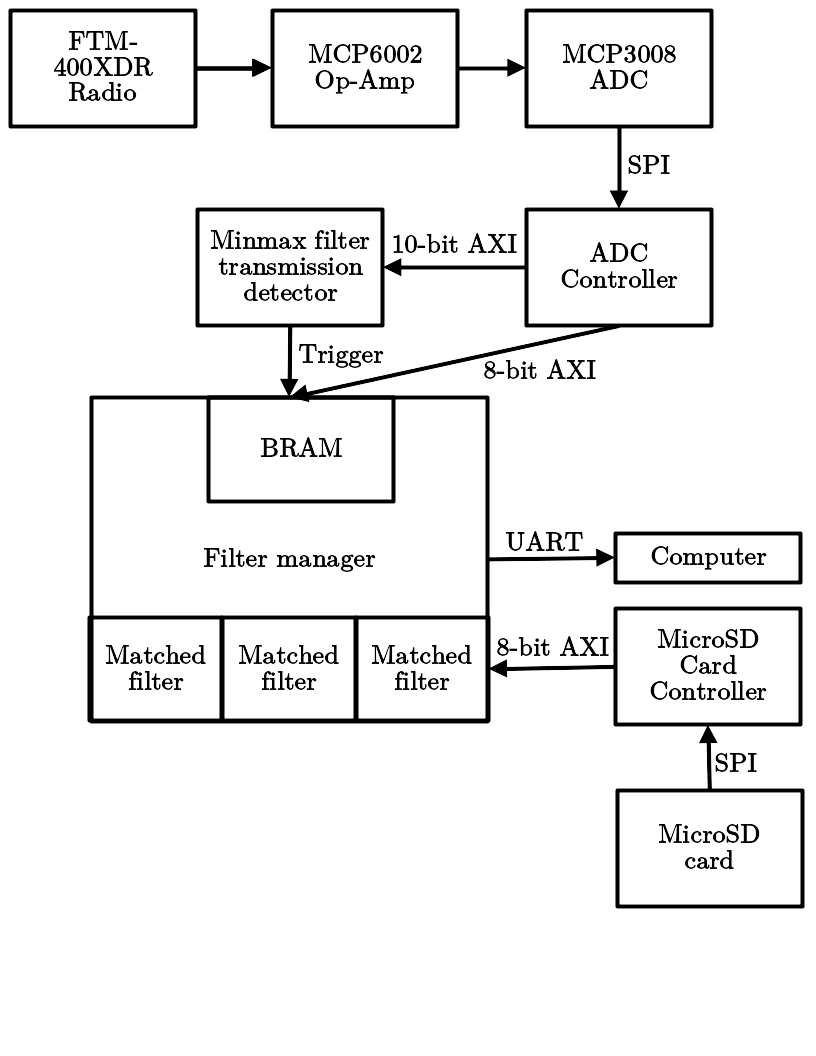
\includegraphics[width=\textwidth]{Block_Diagram.png}
    \caption{Full system block diagram}
    \label{block_diagram}
\end{figure*}

\begin{thebibliography}{00}
\bibitem{b1} B. Fields, ``Transmitter fingerprinting," W9CR, 19-Nov-2020. [Online]. Available: https://wiki.w9cr.net/index.php/Transmitter\_Fingerprinting. [Accessed: 23-Nov-2022].

\bibitem{b2} R. Rager, ``XMIT\_ID version 2.61," XMIT ID version 2.61, 15-Nov-2000. [Online]. Available: https://www.qsl.net/n9zia/xmit\_id/index.html. [Accessed: 23-Nov-2022].
\end{thebibliography}

\vspace{12pt}

\end{document}
